\documentclass[10pt, conference]{IEEEtran}
\IEEEoverridecommandlockouts
% The preceding line is only needed to identify funding in the first footnote. If that is unneeded, please comment it out.
\usepackage{cite}
\usepackage{amsmath,amssymb,amsfonts}
\usepackage{algorithmic}
\usepackage{graphicx}
\usepackage{textcomp}
\usepackage{xcolor}
\def\BibTeX{{\rm B\kern-.05em{\sc i\kern-.025em b}\kern-.08em
    T\kern-.1667em\lower.7ex\hbox{E}\kern-.125emX}}
\begin{document}

\title{ManyTypes4Py: A benchmark dataset for machine learning-based type inference\\
%{\footnotesize \textsuperscript{*}Note: Sub-titles are not captured in Xplore and
%should not be used}
%\thanks{Identify applicable funding agency here. If none, delete this.}
}

\author{\IEEEauthorblockN{Amir M. Mir}
\IEEEauthorblockA{\textit{Department of Software Technology} \\
\textit{Delft University of Technology}\\
Delft, The Netherlands \\
s.a.m.mir@tudelft.nl}
\and
\IEEEauthorblockN{Evaldas Latoškinas}
\IEEEauthorblockA{\textit{Department of Software Technology} \\
\textit{Delft University of Technology}\\
Delft, The Netherlands \\
e.latoskinas@student.tudelft.nl}
\and
\IEEEauthorblockN{Georgios Gousios}
\IEEEauthorblockA{\textit{Department of Software Technology} \\
\textit{Delft University of Technology}\\
Delft, The Netherlands \\
g.gousios@tudelft.nl}
}

\maketitle

\begin{abstract}

\end{abstract}

\begin{IEEEkeywords}
\end{IEEEkeywords}

\section{Introduction}

\begin{figure*}[!t]
	\centering
	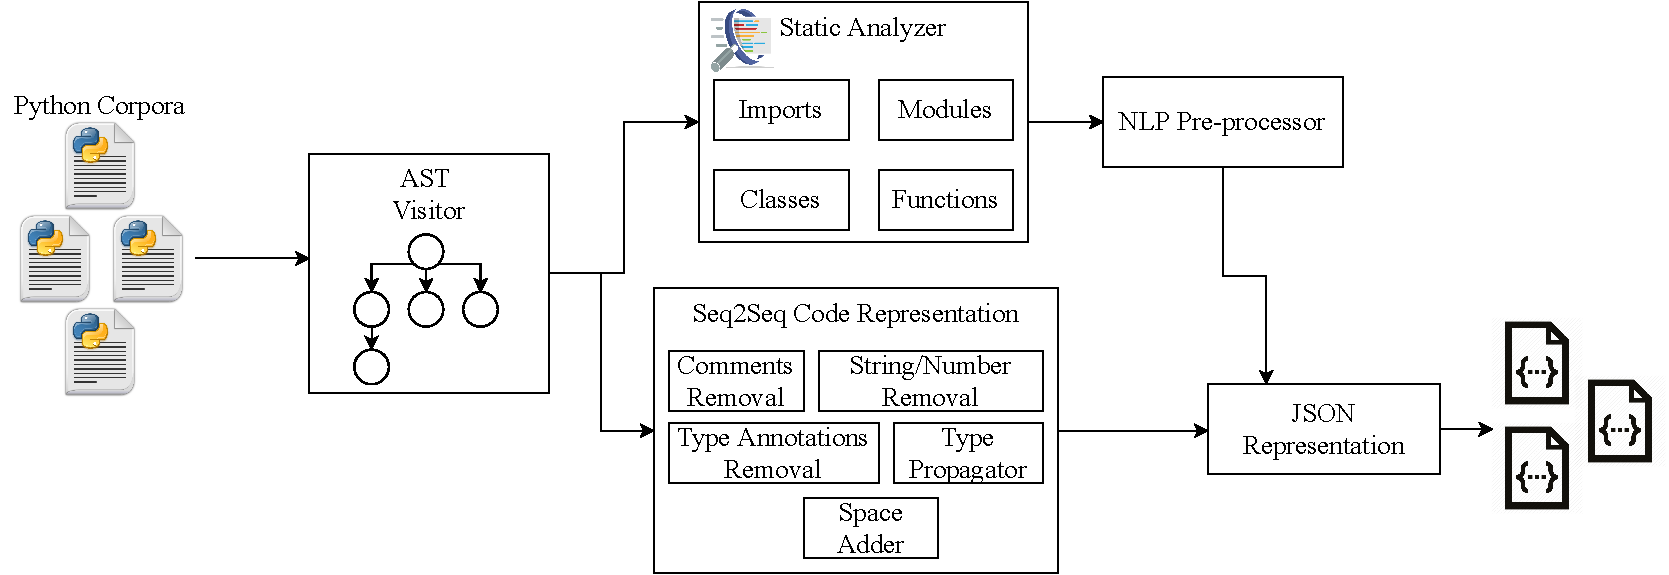
\includegraphics[width=\linewidth]{figs/manytypes4py-pipeline.pdf}
	\caption{Overview of light-weight static analysis pipeline}
	\label{fig:overview-pipeline-sa}
\end{figure*}

\section{Methodology}
We created ManyType4Py dataset using the following methodology:

\begin{itemize}
	\item To find Python projects with type annotations, we intuitively search for projects that has mypy as a depdendency on libraries.io. Since mypy is the most used type checker for Python, projects that use mypy have most likely type annotations. Our search resulted in 5,382 Python projects that are publicly available on GitHub. We cloned all the discovered projects on the disk in Sep. 2020 and finally created a file that contains projects' URL and their latest commit hash. The resulting dataset is roughly 60 GB in size before pre-processing.
	\item As demonstrated by Allamanis \cite{allamanis2019adverse}, it is essential to de-duplicate a code corpora. Because code duplication negatively affects the performance of machine learning models when testing on duplicated code corpora. Following this, we de-duplicated the collected Python corpora in the previous step using our code de-duplication tool, namely, CD4Py\footnote{https://github.com/saltudelft/CD4Py}. In short, the CD4Py tool tokenizes Python source code files, vectorizes files using term frequency-inverse document (TF-IDF), and performs $k$-nearest neighbor search to identify candidate duplicates files. Out of 636,383 Python source code files, 354,409 files were identified as duplicate and they are removed from the code corpora.
	\item After the removal of duplicate files, we split the Python code corpora into three sets by files, i.e., 70\% training data, 10\% validation data, and 20\% test data. This is a common practice that is considered in recent research work \cite{pradel2019typewriter, allamanis2020typilus}, concerning machine learning-based models for type inference.
	% file extensions removal might worth mentioning here
	\item Given the de-duplicated code corpora and a list of files for the three sets, we ran our light-weight static analysis pipeline, which is depicted in Figure \ref{fig:overview-pipeline-sa}. First, the Abstract Syntax Tree (AST) of Python source files are extracted and nodes in ASTs are visited. Second, using the light-weight static analyzer, type-related information are extracted from imports, modules, classes, and functions. Third, the seq2seq representation of source code files \cite{hellendoorn2018deep} are generated by removing comments, string, number literals, and propagating types. Forth, common NLP practices such as tokenization and lemmatization are applied to idenfier names in source code files. Finally, the processed Python projects are stored as a JSON-formatted file which is described in ?. 
\end{itemize}



\section{Description}

\section{Applications}

\section{Benchmark}

\section{Related Work}
There are a number of Python code copora that can be used for machine learning-based type inference. Recently, Allamanis et al. \cite{allamanis2020typilus} proposed Typilus model, which is a graph-based neural model that predicts type annotations for Python. The Typilus model \cite{allamanis2020typilus} accompanies with a relatively small dataset which contains 600 Python projects. Moreover, the source code files of Typilus' dataset is converted to graph representations that is onlu suitable for training the Typilus model. However, the ManyTypes4Py dataset provides JSON-formatted analyzed source code files that contains useful type hints for training various machine learning models.


\section{Conclusion}

\section*{Acknowledgment}

\section*{References}

\bibliographystyle{IEEEtran}
\bibliography{main}

\end{document}
